Parameters used in logistic regression :
\vspace{0.5cm}

{
\renewcommand{\arraystretch}{1.5}
\begin{tabular}{ccl}
	$n_x$ & : &  number of features \\
	$x\in\mathbb{R}^{n_x}$ & : & input features vector \\
	$y\in\{0,1\}$ & : & training label \\
	$w\in\mathbb{R}^{n_x}$ & : & weights \\
	$b\in\mathbb{R}$ & : & threshold \\
	$\hat{y} = \sigma(w^T x + b)$ & : & the output \\
	$\sigma(z) = \frac{1}{1+\exp(-z)}$ & : & sigmoid function \\
	$\mathcal{L}(y,\hat{y}) = -y \log(\hat{y}) - (1-y) \log(1-\hat{y})$ & :& cost function (single example)
\end{tabular} 
}

See Figure~\ref{fig:sigmoid} for an illustration of the sigmoid function.

\begin{figure}[h]
	\centering
	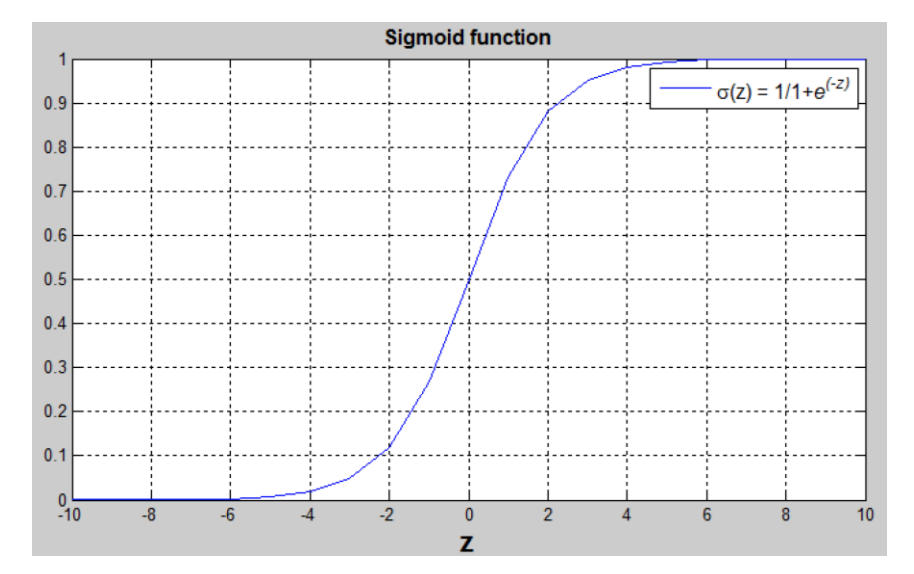
\includegraphics[scale=0.5]{sigmoid_function.png}
	\caption{\label{fig:sigmoid}Sigmoid function}
\end{figure}

Since we have multiple examples, we take the mean over all examples for this cost function.
Let $m$ be the number of examples.

\begin{align}
	Y,\hat{Y}&\in\mathbb{R}^{1\times m} \\
	J(Y, \hat{Y})  &= \frac{1}{m} \sum_{i=1}^{m} \mathcal{L}(Y^{(i)},\hat{Y}^{(i)}) \\
	&= \frac{-1}{m} \sum_{i=1}^{m} \left(
	Y^{(i)} \log(A^{[L](i)}) + (1-Y^{(i)}) \log(1 - A^{[L](i)})
	\right)
\end{align}

\subsection{Regularization}
\subsubsection{$L_2$ regularization}
We have $W\in\mathbb{R}^{1\times n_x}$.
The cost function becomes as follows.
\begin{align}
	J(Y, \hat{Y})
		&= \frac{1}{m} \sum_{i=1}^{m} \mathcal{L}(Y^{(i)},\hat{Y}^{(i)}) + \frac{\lambda}{2m} || W ||_2^2 \\
		&= \frac{1}{m} \sum_{i=1}^{m} \mathcal{L}(Y^{(i)},\hat{Y}^{(i)}) + \frac{\lambda}{2m} \sum_{k=1}^{n_x} W_k^2
\end{align}

\subsubsection{$L_1$ regularization}
The cost function becomes as follows.
\begin{align}
	J(Y, \hat{Y})
		&= \frac{1}{m} \sum_{i=1}^{m} \mathcal{L}(Y^{(i)},\hat{Y}^{(i)})  + \frac{\lambda}{2m} || W ||_1 \\
		&= \frac{1}{m} \sum_{i=1}^{m} \mathcal{L}(Y^{(i)},\hat{Y}^{(i)})  + \frac{\lambda}{2m} \sum_{k=1}^{n_x} | W_k |
\end{align}
